\subsection*{Six-property conditioning does not remove the frontier bottleneck}

To test whether the limitation was specific to a single scalar label, we evaluated a parallel six-property conditioning benchmark on the Q80 intersection (2,494 of 6,024 rows). The joint target vector comprised conductivity, lithium diffusivity, TFSI diffusivity, polymer diffusivity, transference number and molality. The benchmark compared multi-property conditioning with scalar-conductivity conditioning, binary conditioning and unconditional reranking.

Across Q90, Q100, train-max+0.25 and train-max+0.50, no arm produced a strict joint hit or an all-six-property frontier crossing. The result is consistent with the scalar experiment: increasing the number of conditioning coordinates improves the specification of the target, but does not create training support where none exists.

\begin{figure}[H]
\centering
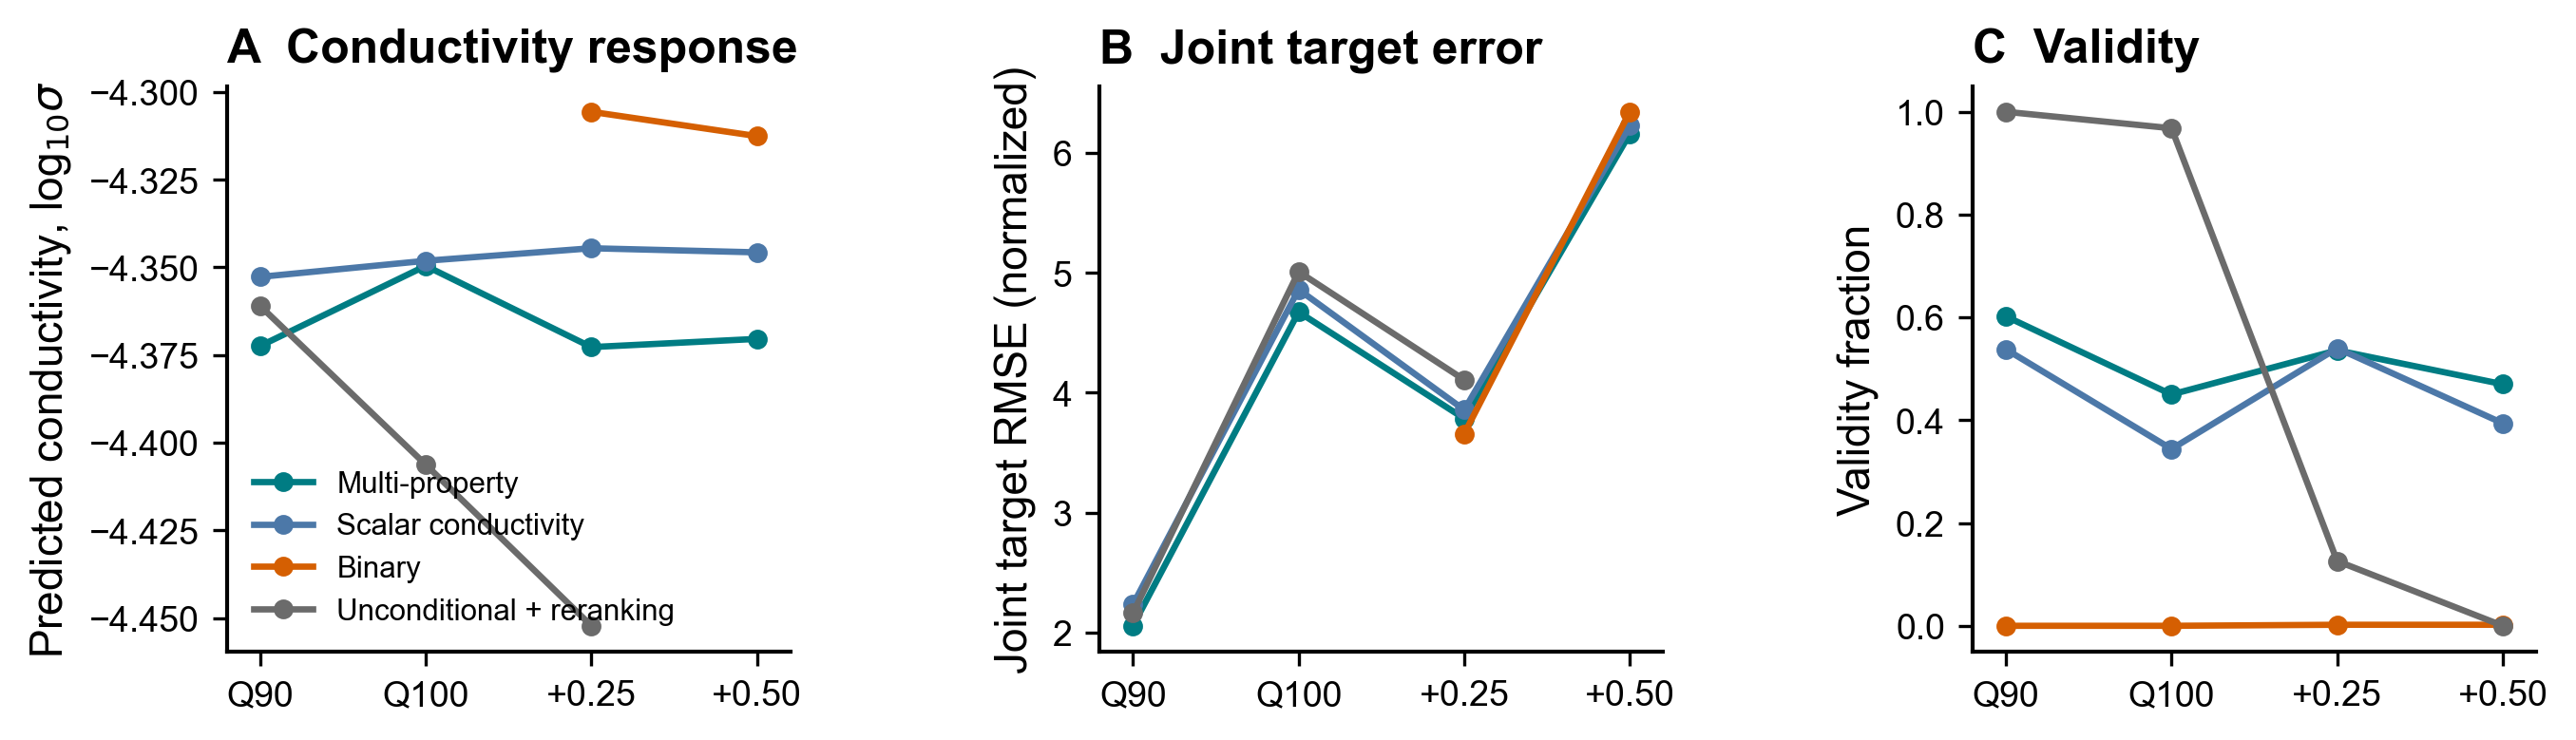
\includegraphics[width=0.98\linewidth]{figures/Figure_1_multi_property_response.png}
\caption{Joint-property extrapolation response. Multi-property conditioning produces no strict joint hit or all-property frontier crossing in the extrapolation regions.}
\label{fig:multi-property-response}
\end{figure}

This parallel result is particularly important for interpreting multi-property generation papers. A richer conditioning vector can enable in-support re-ranking or target trade-offs without establishing out-of-support generalization. Here, the all-property frontier criterion makes that distinction explicit.
